\documentclass[12pt, a4paper]{article}


% A pretty common set of packages
\usepackage[margin=2.5cm]{geometry}
\usepackage[T1]{fontenc}
\usepackage{graphicx}
\usepackage{amssymb}
\usepackage{amsmath}
\usepackage{color}
\usepackage{booktabs}
\usepackage{multirow}
\usepackage{engord}
\usepackage{soul}
\usepackage{textcomp}
\usepackage{parskip}
\usepackage{setspace}
\usepackage{titlesec}
\usepackage{fancyhdr}
\pagestyle{fancy}
\usepackage[UKenglish]{babel}
\usepackage[UKenglish]{isodate}
\usepackage[skip=2pt,font=footnotesize,justification=centering]{caption}
\usepackage{natbib}
\usepackage[colorlinks=true, 
    linkcolor=blue,          % color of internal links
    citecolor=blue,        % color of links to bibliography
    filecolor=blue,      % color of file links
    urlcolor=blue]{hyperref}




% Do you prefer Sans Serif fonts?
%\usepackage{sfmath}
%\renewcommand{\familydefault}{\sfdefault} 




% Make some additional useful commands
\newcommand{\ie}{\emph{i.e.}\ }
\newcommand{\eg}{\emph{e.g.}\ }
\newcommand{\etal}{\emph{et al}}
\newcommand{\sub}[1]{$_{\textrm{#1}}$}
\newcommand{\super}[1]{$^{\textrm{#1}}$}
\newcommand{\degC}{$^{\circ}$C}
\newcommand{\wig}{$\sim$}
\newcommand{\ord}[1]{\engordnumber{#1}}
\newcommand{\num}[2]{$#1\,$#2}
\newcommand{\range}[3]{$#1$-$#2\,$#3}
\newcommand{\roughly}[2]{$\sim\!#1\,$#2}
\newcommand{\area}[3]{$#1 \! \times \! #2\,$#3}
\newcommand{\vol}[4]{$#1 \! \times \! #2 \! \times \! #3\,$#4}
\newcommand{\cube}[1]{$#1 \! \times \! #1 \! \times \! #1$}
\newcommand{\figref}[1]{Figure~\ref{#1}}
\newcommand{\eqnref}[1]{Equation~\ref{#1}}
\newcommand{\tableref}[1]{Table~\ref{#1}}
\newcommand{\secref}[1]{Section \ref{#1}}
\newcommand{\XC}{\emph{exchange-correlation}}
\newcommand{\abinit}{\emph{ab initio}}
\newcommand{\Abinit}{\emph{Ab initio}}
\newcommand{\Lonetwo}{L1$_{2}$}
\newcommand{\Dznt}{D0$_{19}$}
\newcommand{\Dtf}{D8$_{5}$}
\newcommand{\Btwo}{B$_{2}$}
\newcommand{\fcc}{\emph{fcc}}
\newcommand{\hcp}{\emph{hcp}}
\newcommand{\bcc}{\emph{bcc}}
\newcommand{\Ang}{{\AA}}
\newcommand{\inverseAng}{{\AA}$^{-1}$}
%\newcommand{\comment}[1]{}
\newcommand{\comment}[1]{\textcolor{red}{[COMMENT: #1]}}
\newcommand{\more}{\textcolor{red}{[MORE]}}
\newcommand{\red}[1]{\textcolor{red}{#1}}





% Change this to modify look of header and footer
\lhead{}
\chead{}
\rhead{}
\lfoot{}
\cfoot{\thepage{}}
\rfoot{}
\renewcommand{\headrulewidth}{0pt}
\renewcommand{\footrulewidth}{0pt}



\begin{document}

\onehalfspacing


\begin{titlepage}

\begin{center}

\includegraphics[width=1in]{figures/bham_crest}

\vspace{0.3in}


\includegraphics[width=3in]{figures/bham_logo}

\vspace{2in}

{\LARGE The project title of my individual research project }

\vspace{0.7in}

{\Large A. Student (123456)}


\vfill{}
Final project report submitted\\ 
in partial fulfilment for the degree of\\
M.ENG. IN NUCLEAR ENGINEERING
\end{center}

\vspace{0.4in}
Date: \today{}     \hfill{} Project supervisor: \\
Word count: 7,999   \hfill{} Dr Alessandro Mottura
\end{titlepage}






\tableofcontents

\newpage{}










\section{Abstract}
A summary of the scope and significance of the project, the methodology / techniques used, the results gained / outcomes generated and the conclusions obtained. Abstracts are generally a single paragraph and less than 250 words.





\section{Introduction}
An introduction to the project -- your aims and objectives should go here. You can use bullet points. You probably want to keep this to half-page or so.



\section{Literature review}
This should demonstrate a sound understanding of the current state of knowledge in the field, which should critically assess previous and current work in the public domain, drawing out the major facts, views, trends etc. (not just listing a series of literature / information sources and/or literature/ information abstracts). 

This should then develop into a description of the need for the project and so define the
project aims and how they are to be attained in the methodology and/or experimental work. Literature in \LaTeX{} \citep{ardell05} is best done using BibTeX \citep{ashbyjones, hk}. For your individual project you are asked to use the Harvard method for citations -- \LaTeX{} can do it very easily (see above).







\section{Methodology}
Description of the methodology and/or experimental methods used to achieve aims of the project in sufficient detail to allow other researchers to repeat your work.





\section{Results}
This should be a coherent presentation of the results / outcomes of your work, including your methodology and/or experimental work, such that the key findings i.e. facts, views, trends etc. are readily revealed (this should not be a chronological presentation of what was carried out nor, usually, just the raw data).

\begin{figure}
\begin{center}
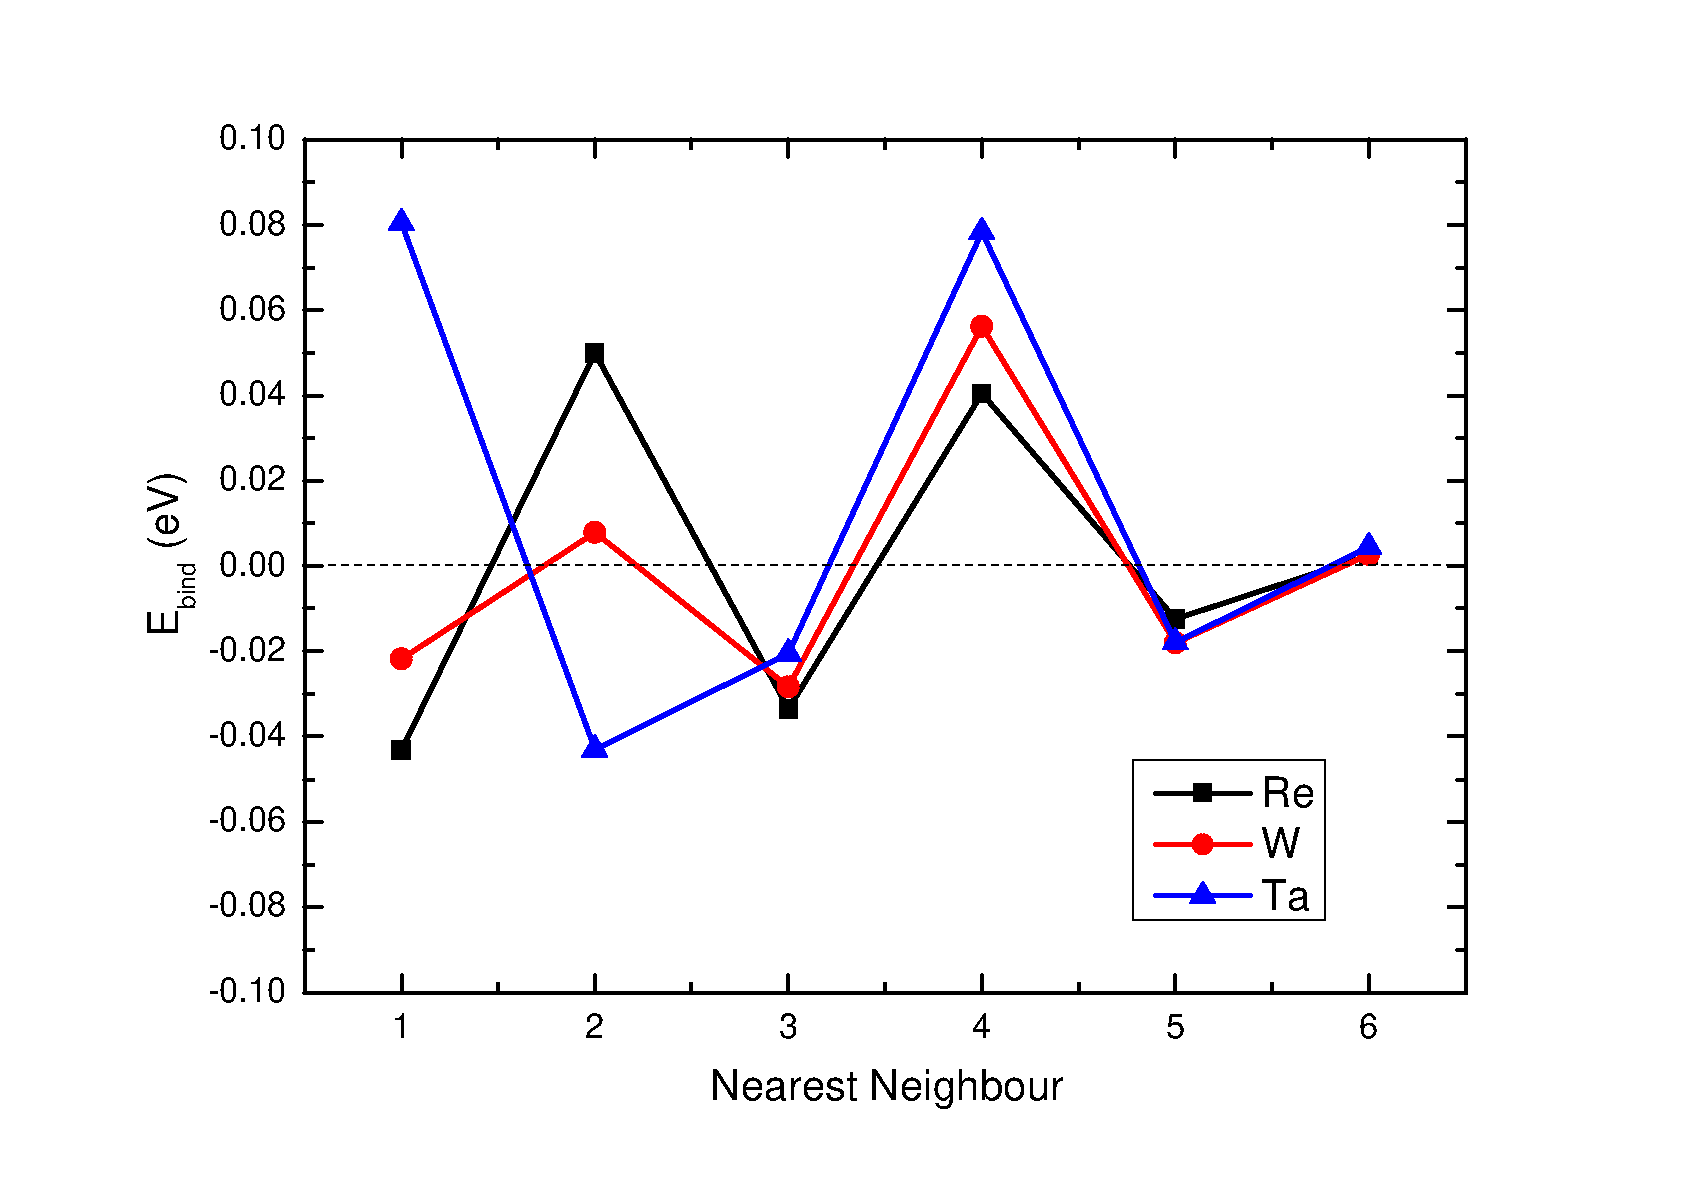
\includegraphics[width=4in]{figures/examplefig}
\caption{Some example figure}
\label{examplefig}
\end{center}
\end{figure}

A good example of how to insert a figure in \LaTeX{} is shown in \figref{examplefig}. Note that in \LaTeX{} all figures are \emph{floats}. This means they are items that flow all the way to the top of the page.








\section{Discussion}
An analysis of the results of your methodology and/or experimental work, relating the findings back to the assessment of current state of understanding presented in the introduction.






\section{Conclusiones}
A well-defined summary of the major findings and their interpretation (this should not be further discussion of the results or speculate on areas not assessed in the results and discussion).



\section{Bibliografía}

[1] T. Kim, "CSI-Chain: A Complete End-to-End Framework for WiFi CSI Sensing" Mar. 31, 2026. KSII Transactions on Internet and Information Systems: 10.3837/tiis.2026.03.008

[2] B. Barahimi, “Context-Aware Predictive Coding: A Representation Learning Framework for WiFi Sensing,” IEEE Journals and Magazine | IEEE Xplore: 10.1109/OJCOMS.2024.3465216

[3] O. Custance and others, “Why Commodity WiFi Sensors Fail at Multi-Person Gait Identification: A Systematic Analysis Using ESP32,” \emph{arXiv preprint arXiv:2601.02177}, 2026, doi: 10.48550/arXiv.2601.02177.

[4] P.Mykytyn, “Channel State Information Analysis for jamming attack detection in static and dynamic UAV networks – an experimental study,” IEEE Conference Publication | IEEE Xplore: 10.1109/DCOSS-IoT65416.2025.00060


[5] S. Hernandez, “Extract Channel State Information from WiFi-enabled ESP32 Microcontroller. Active and Passive modes available: https://github.com/StevenMHernandez/ESP32-CSI-Tool

[6] S. Gaire and others, “StaticSense: Static Object Detection using Wi-Fi Channel State Information,” \emph{IEEE}, 2026, doi: 10.1109/ICTP67998.2026.11485253

[7] D. Avola et al., “Transformer-Based Person Identification via Wi-Fi CSI Amplitude and Phase Perturbations,” \emph{arXiv preprint arXiv:2507.12854}, 2025, doi: 10.48550/arXiv.2507.12854

%\bibliographystyle{chicago}
%\bibliography{Literature}
%\end{thebibliography}



\end{document}



